\section{Results}
\label{sec:results}

\subsection{Released per-skill evidence certifies few skills sequentially}
\label{sec:res-real}

\paragraph{SWE-Skills-Bench (E8).} The source paper's rule (exact two-sided sign-flip test on the ten batch differences, $p<0.05$) marks \NSweGolden{} of the \NSweCells{} skill-by-configuration cells, covering \NSweGoldenSkills{} skills, as golden and \NSweHarmful{} as harmful. None of the one-sided $p$-values survives Benjamini-Hochberg control at 5\% (\NSweBH{} admissions), and no betting test admits any cell. With ten units admission needs a nearly perfect record: the grid bet admits after \NSweGridMinAllOnes{} straight wins, but no cell's wealth passed \NSweObsWealthGrid{} of the 20 needed (Appendix~\ref{app:more}). Pooling a skill's 40 units across configurations, \NSwePooled{} skills pass an uncorrected one-sided test, \NSwePooledBH{} after correction, and \NSwePooledBet{} the grid betting test (\NSwePooledBetPrpl{} with PrPl). The uncorrected calls are not noise: cells flagged on one configuration show a mean lift of \NSweRepLift{} points on the other three, positive for \NSweRepPos\% of them against \NSweAllPos\% of all cells. Admitting a skill that passes on any of the four configurations raises the false-admission rate on the sign-flip null from \NShopPer\% to \NShopAny\%.

\paragraph{SkillsBench (E9).} With 18 paired units per curated skill, a one-sided $t$-test admits \NSbT{} of \NSbTasks{} skills, \NSbTBH{} after Benjamini-Hochberg correction; the grid betting test admits \NSbBet{} (PrPl: \NSbBetPrpl{} with cap $1/2$, \NSbBetHi{} with cap $3/4$), and e-BH on the final grid wealth admits \NSbEBH{} (PrPl: \NSbEBHPrpl). Splitting the configurations into random halves 500 times, skills admitted on one half (\NSbSplitAdm{} on average) show \NSbSplitLift{} points of lift on the other, positive in \NSbSplitPos\% of cases, against \NSbSplitNot{} points for skills not admitted. Benjamini-Hochberg admissions replicate even better (\NSbSplitBHAdm{} on average, \NSbSplitBHLift{} points, \NSbSplitBHPos\% positive). Other valid fixed-sample procedures agree (E10, Appendix~\ref{app:more}). A one-off fixed-sample analysis of a completed benchmark can therefore certify a share of skills. A registry cannot use it as its decision rule, because skills arrive over time, exams are stopped when results look good, and authors resubmit (Section~\ref{sec:res-validity}); the anytime-valid procedure that survives those conditions, e-LOND over skills in arrival order with the grid bet, certifies \NSbELond{} skills on average with 18 units (\NSbELondLo{} to \NSbELondHi{} over 90\% of random orders; Bonferroni at $\alpha/87$: \NSbBonfBet; none with PrPl), against \NSbTBH{} for the one-off analysis. The obstacle is sample size (Section~\ref{sec:res-cost}).

\subsection{Validity under optional stopping}
\label{sec:res-validity}

Table~\ref{tab:false} gives false-admission rates under nulls (Figure~\ref{fig:false} in Appendix~\ref{app:more} plots them). Re-checking a $t$-test after every variant admits up to \NEOnePeekTMax\% of useless skills, and re-checking a 95\% interval every ten variants up to \NEOnePeekCIMax\% (the lowest rates, \NEOnePeekTMin\% and \NEOnePeekCIMin\%, are for a slightly harmful placebo skill not shown in the table); at the null boundary the interval rule runs at \NEOnePeekRatio{} times 5\%, and twice that relative to its one-sided level of 2.5\%; on the resampled SWE-Skills-Bench null the rates are \NEEightNullPeekT\% and \NEEightNullPeekCI\%. The fixed-$n$ test holds its level (\NEOneFixed\% at the boundary). The SPRT, the mSPRT and every betting variant stay within Monte Carlo error of 5\% or below in every null configuration, including the worst case in which every pair is discordant. The largest rate among them is \NEOneValidMax\% (standard error \NEOneValidMaxSE), for the SPRT with common random numbers at $\rho=0.9$ (Appendix~\ref{app:more}); the betting gates stay below 3.5\%.

The last column changes the comparison rather than the test: the comparator arm comes from a stored run and the provider's model has since improved by \PDrift{} logit units, while the skill has no effect. Every gate then admits \NEOneStaleMin\% to \NEOneStaleMax\% of the time, the betting gate included (\NEOneStaleBet\%), because a stale baseline violates the condition of Proposition~\ref{prop:valid}. Running the arms concurrently matters more than the choice of test.

\begin{table}[t]
\centering\small
\caption{False-admission rate (\%) by gate and null configuration (E1, E8). Boundary: $\Delta=\delta=0$ under the default model. Worst case: every pair discordant. Stale baseline: the comparator arm is from an earlier model snapshot. SWE null: the SWE-Skills-Bench differences with random signs. Dashes: the discordant-pair SPRT is defined only for one pass/fail attempt per arm at $\delta=0$, so it is not run with $r=3$, with a margin, or on batch pass rates.}
\label{tab:false}
\resizebox{\linewidth}{!}{\begin{tabular}{lrrrrrrrr}
\toprule
Gate & Boundary & Worst case & $s_\theta=3$ & $\rho=0$ & $r=3$ & $\delta=0.05$ & Stale baseline & SWE null \\
\midrule
Fixed-$n$ paired $t$ & 4.9 & 4.3 & 5.1 & 5.2 & 5.0 & 5.1 & 65.4 & 3.3 \\
$t$-test re-checked each variant & 32.0 & 34.5 & 30.2 & 33.9 & 33.8 & 30.7 & 98.7 & 30.3 \\
95\% CI re-checked every 10 & 18.1 & 18.9 & 16.2 & 19.9 & 19.2 & 16.7 & 96.8 & 15.4 \\
SPRT, discordant pairs & 4.3 & 4.2 & 4.9 & 4.6 & -- & -- & 69.7 & -- \\
mSPRT & 1.3 & 1.3 & 0.9 & 1.6 & 2.2 & 1.4 & 75.6 & 0.5 \\
Betting, cap $\lambda\le m_0$ & 1.5 & 2.7 & 0.9 & 2.1 & 0.5 & 1.9 & 75.4 & 0.2 \\
Betting, $c=1/2$ & 1.5 & 2.7 & 0.9 & 2.1 & 0.5 & 1.8 & 75.4 & 0.2 \\
Betting, $c=3/4$ & 2.2 & 3.3 & 1.8 & 2.8 & 1.3 & 2.5 & 69.7 & 0.8 \\
Betting, aGRAPA & 2.1 & 2.6 & 1.9 & 2.4 & 1.7 & 2.3 & 73.0 & 1.3 \\
Betting, $c=1/2$, futility margin & 1.5 & 2.7 & 0.9 & 2.1 & 0.5 & 1.8 & 75.4 & 0.2 \\
Betting, grid (deployed) & 2.7 & 2.8 & 2.6 & 2.9 & 3.0 & 3.3 & 66.3 & 2.8 \\
Betting, grid, futility margin & 2.7 & 2.8 & 2.6 & 2.9 & 3.0 & 3.3 & 66.2 & 2.2 \\
\bottomrule
\end{tabular}
}
\end{table}

\subsection{What validity costs}
\label{sec:res-cost}

\paragraph{Matched power (E18).} Comparing gates at different power mixes cost with power, so E18 tunes each gate to the same power: the fixed-$n$ test by its sample size, the SPRT by $\beta$, and the truncated sequential gates by the smallest $N_{\max}$ that reaches the target (Table~\ref{tab:matched}). At 80\% power the deployed grid gate costs about what a fixed-$n$ test costs when the skill helps (\NMpDesEightyGrid{} against \NMpDesEightyFixed{} variants at the design lift, \NMpCurEightyGrid{} against \NMpCurEightyFixed{} at the curated lift); at 95\% it is cheaper (\NMpDesNinetyFiveGrid{} against \NMpDesNinetyFiveFixed, and \NMpCurNinetyFiveGrid{} against \NMpCurNinetyFiveFixed), because early stopping pays more when the fixed design must cover the tail. The price of anytime validity falls on useless skills: at the 80\% design the grid gate spends \NMpDesEightyGridNull{} variants on a useless skill against \NMpDesEightyFixedNull{} for the fixed design. The discordant-pair SPRT is cheapest where it applies (pass/fail scores, $r=1$, no margin), and PrPl with cap $1/2$ is the most expensive betting rule. The same ordering holds for $r=3$ and for the moment-matched model (Appendix~\ref{app:more}); the tuned grid gate never admitted a useless skill more than \NMpNullMaxGrid\% of the time.
\begin{table}[t]
\centering\small
\caption{Expected variants at matched power (E18; default model, $r=1$, 4{,}000 exams per cell): when the skill has the stated lift, and in parentheses for a useless skill ($\Delta=0$) with the same tuning. The SPRT assumes pass/fail scores and no margin.}
\label{tab:matched}
\begin{tabular}{llrrrrr}
\toprule
Lift & Power & Fixed-$n$ & SPRT & mSPRT & PrPl & Grid \\
\midrule
0.1 & 80\% & 137 (137) & 96 (76) & 167 (278) & 167 (219) & 148 (227) \\
0.1 & 95\% & 239 (239) & 124 (141) & 183 (427) & 183 (297) & 167 (313) \\
0.166 & 80\% & 55 (55) & 41 (38) & 76 (120) & 87 (116) & 57 (97) \\
0.166 & 95\% & 96 (96) & 57 (70) & 81 (164) & 91 (149) & 64 (147) \\
\bottomrule
\end{tabular}

\end{table}

Figure~\ref{fig:power} shows power and expected variants. At the design lift of \PLiftOne{} points the fixed-$n$ test has \NETwoPowFixed\% power with \NFixedN{} variants; the betting gate with futility margin has \NETwoPowBet\% power with \NETwoNBetLOne{} variants on average, and at the SkillsBench curated average (\PCurated{} points) it stops after \NETwoNBetCur{}, \NETwoSaveCur\% fewer than the fixed design. Anytime validity costs variants near the design lift and saves them above it. The futility margin cuts the variants a useless skill consumes from \NETwoNBetZero{} to \NETwoNBetFutZero. Across the default and moment-matched models with $\kappa\in\{-0.5,0,0.5\}$ (E14, $r=1$), the fixed design needs \NRvSensNFixedLo{} to \NRvSensNFixedHi{} variants, and the betting gate uses \NRvSensNBetLo{} to \NRvSensNBetHi{} at the design lift (power at least \NRvSensPowBetLo\%) and \NRvSensNCurLo{} to \NRvSensNCurHi{} at the curated lift, \NRvSensSaveLo\% to \NRvSensSaveHi\% fewer than the fixed design. No model raises the betting gate's false-admission rate above \NRvSensNullMax\%. At $r=3$ the moment-matched model raises the betting gate's variants at the design lift from \NRvDefRThreeNBet{} to \NRvFitRThreeNBet.

\paragraph{Where the betting gate loses.} Three regimes favour other designs. With a margin $\delta=0.05$, the betting gate has \NRvMarginPowBet\% power at the design lift against \NRvMarginPowFixed\% for a fixed-$n$ test planned for the margin (\NRvMarginNFixed{} variants, against \NRvMarginNBet{} on average for the betting gate), because only five points of lift lie above the margin and the bets are capped. With $r=3$ attempts per arm the differences are less noisy: the fixed design needs only \NRvRThreeNFixed{} variants for \NRvRThreePowFixed\% power, while the betting gate, with higher power, uses \NRvRThreeNBet{} on average. For pass/fail scores at $\delta=0$, the discordant-pair SPRT is cheaper at matched power (E14). At the design lift it reaches \NRvSprtPowLow\% power with \NRvSprtNLow{} variants, where the betting gate with futility, truncated at \NRvBetNMaxLow{} variants, reaches \NRvBetPowLow\% with \NRvBetNLow. At \NRvSprtPowHigh\% power the SPRT needs \NRvSprtNHigh{} variants, the betting gate \NRvBetNHigh{} and a fixed-$n$ test \NRvFixedNHigh (here the cap is fixed; Table~\ref{tab:matched}, from E18, instead tunes each gate's cap to the target power). The SPRT gains by assuming the form of the alternative, and it does not apply to graded scores, to $r>1$ or to a margin. Anytime validity is therefore not free. It pays when lifts are well above the design lift and when exams are monitored, stopped early or resumed, and it costs power when the margin is close to the lift.

\begin{figure}[t]
\centering
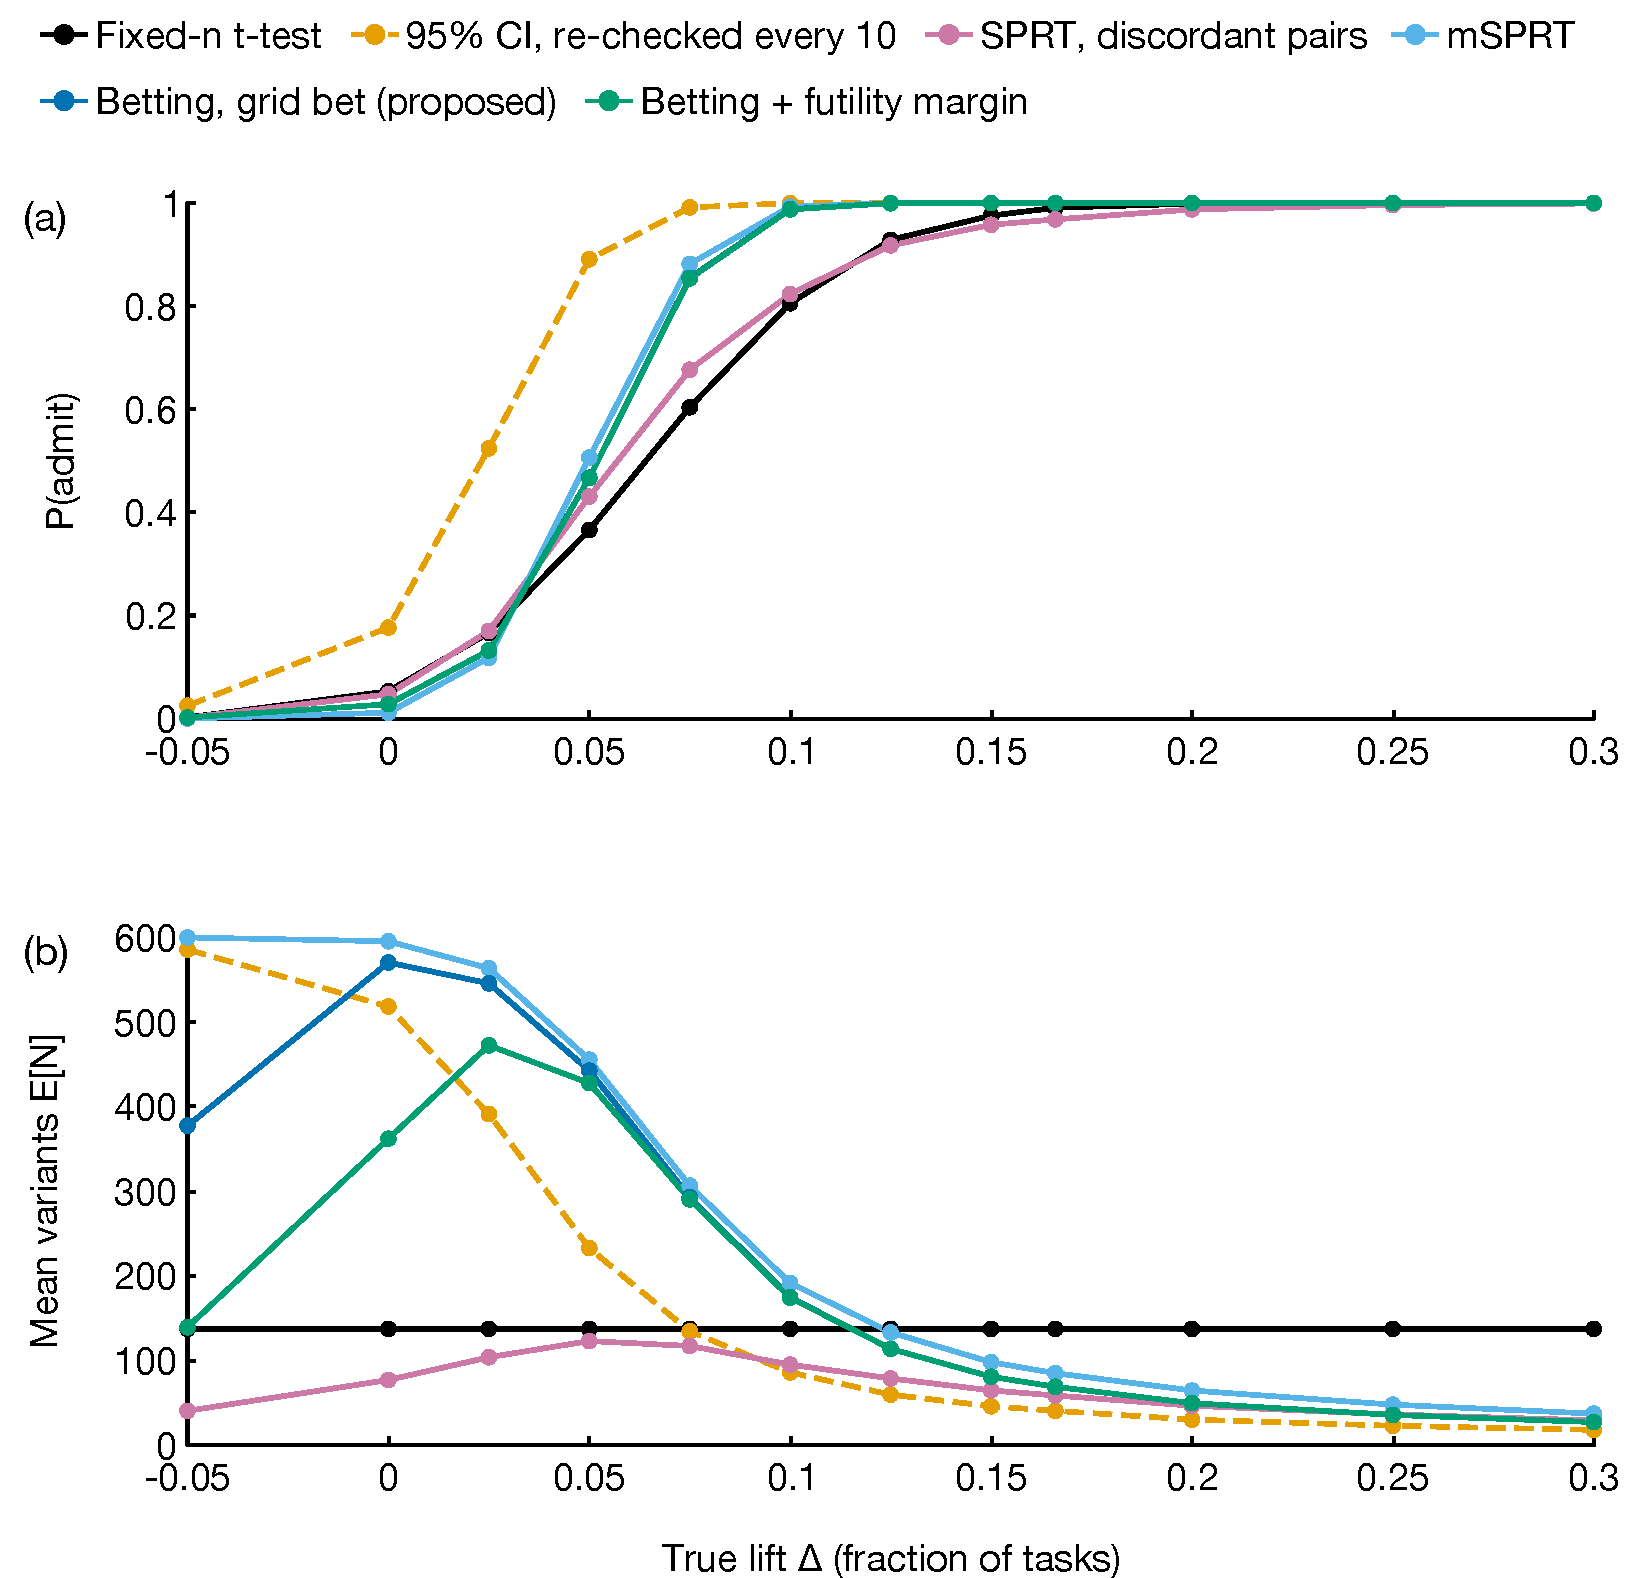
\includegraphics[width=0.78\linewidth]{F3_power_cost.pdf}
\caption{(a) Admission probability and (b) mean variants per exam against the true lift (E2, \PRepsPower{} replicates per point, $N_{\max}=\PNmax$). The re-checked interval (dashed) is fast because it is invalid.}
\label{fig:power}
\end{figure}

In libraries whose lifts follow the published benchmark summaries (E5, Table~\ref{tab:scen} in Appendix~\ref{app:more}), the cost is dominated by useless candidates. In a SWE-like library, where 94\% of skills have no effect, \NEFiveSweFalseFixed\% of the skills admitted by an uncorrected fixed-$n$ test are useless, \NEFiveSweFalsePeekCI\% for the re-checked interval, \NEFiveSweFalseBet\% for the betting gate at a per-exam $\alpha$, and \NEFiveSweFalseELond\% with e-LOND, at \NEFiveSweRunsELond{} agent runs per truly helpful admission.

Resampling each SkillsBench curated skill's 18 per-configuration differences as if they were exam variants, certifying the median helpful skill takes \NSbMedNAlpha{} variants at a per-exam $\alpha$ and \NSbMedNBonf{} at $\alpha/87$ (95\% bootstrap intervals over the skills, \NSbMedNAlphaLo--\NSbMedNAlphaHi{} and \NSbMedNBonfLo--\NSbMedNBonfHi; E24) (Figure~\ref{fig:need} in Appendix~\ref{app:more}); only \NSbCertSix\% are certified within $N_{\max}=600$ at $\alpha/87$. Under the library procedure the gate actually uses, e-LOND with $\gamma_t\propto t^{-1.6}$ over random arrival orders of the 87 skills, the median is \NRvLibELond{} variants (\NRvLibELondCert\% certified within 600), and \NRvLibHorizon{} (\NRvLibHorizonCert\%) when $\gamma_t$ is spread evenly over a planned horizon of 87 (E14). Two assumptions sit behind these numbers. First, the configurations are treated as exchangeable draws of exam variants. They are harness-model pairs, not variants of one task, and we cannot test the assumption. Second, the skills are selected on positive observed lift, which flatters them. Selecting skills on nine configurations and resampling from the same nine gives a median of \NRvSelSame{} variants at $\alpha/87$, against \NRvSelHeld{} when the cost is resampled from the other nine (\NRvSelSameFin\% and \NRvSelHeldFin\% of selected skills certified within 2{,}000; 100 splits, about \NRvSelN{} skills selected). The full-data figures are therefore optimistic. Fixed benchmarks with tens of tasks cannot supply this many paired units per skill; parametric generators can, which is a second reason for hidden variants beyond leakage control.

\subsection{Library error control and resubmission}
\label{sec:res-library}

Table~\ref{tab:lib} reports FDR and power over histories of \PWindows{} windows of \PWindow{} candidates, \PNullShare\% of them useless. Testing each exam at $\alpha$ without correction gives \NEThreeFdrPerExam\% FDR, a figure that grows with the null share. Stopping at $1/\alpha$ and then applying e-BH per window admits nothing (Remark~\ref{prop:ebh}); stopping at $m/\alpha$ or running to $N_{\max}$ restores power at \NEThreeNStopm{} and \NEThreeNRunMax{} variants per exam. e-LOND reaches \NEThreePowELondH\% power at \NEThreeFdrELondH\% FDR with $\gamma_t$ spread over a planned horizon. Over a longer history of \NEbT{} exams (E3b, 60 histories), the deployed $t^{-1.6}$ sequence keeps FDR at \NEbInfFdr{} with \NEbInfPow\% power (rerun with 600 histories: \NIvEbInfFdr\%, 95\% interval up to \NIvEbInfFdrHi\%; E24); power falls from \NEbInfPowFirst\% in the first tenth of the history to \NEbInfPowLast\% in the last; the level $\alpha\gamma_t(R_{t-1}+1)$ grows with the number of earlier admissions, which offsets part of the decay of $\gamma_t$. A known horizon of \NEbT{} gives \NEbHorPow\% power at FDR \NEbHorFdr{}, and testing each exam at $\alpha$ gives \NEbPerPow\% power at FDR \NEbPerFdr{}, above the target. For a first attempt the e-LOND term, not the lineage term, sets the level in \NEbElondBinds\% of exams. With the PrPl bet (cap $1/2$) in place of the grid bet, e-LOND reaches \NEThreePrplPowELond\% power with \NEThreePrplNELond{} variants per exam. A useless skill resubmitted to a per-exam betting gate is admitted within five attempts with probability \NResubFivePerExam\% and within \PResub{} with probability \NResubPerExam\% (\NResubPeekCI\% with a re-checked interval); lineage alpha-spending holds this at \NResubLineage\% (Figure~\ref{fig:resub} in Appendix~\ref{app:more}).

\paragraph{Against stopped e-BH (E20).} Two recent procedures apply e-BH to e-processes directly. Stopped e-BH \citep{wang2025stopped} monitors the e-BH set continuously and controls FDR at any stopping time when the streams are independent; e-BH on suprema adjusted by $A(M)=\sqrt M-1$ \citep{tavyrikov2025carefree} controls FDR under any dependence. We ran both on the E3 histories with the grid bet, letting each exam stop as soon as it enters the e-BH set of its window or at futility. Stopped e-BH reached \NEbhGridSebhPow\% power at \NEbhGridSebhFdr\% FDR with \NEbhGridSebhN{} variants per exam, against \NEbhGridElondPow\% power, \NEbhGridElondFdr\% FDR and \NEbhGridElondN{} variants for the deployed e-LOND in E20's own histories (Table~\ref{tab:lib} reports E3's run of the same rule) (adjusted suprema and the PrPl bet: Appendix~\ref{app:more}). So when candidates arrive in windows whose exams can run side by side, and their data are independent, stopped e-BH is the better library rule. e-LOND remains the rule for a registry that decides each exam as it closes, because it fixes the level when the exam starts and holds under arbitrary dependence; that is the setting of Theorem~\ref{thm:price}, whose levels must be fixed in advance.

\begin{table}[t]
\centering\small
\caption{Library-level control (E3), with the grid bet. Mean over 400 simulated registry histories.}
\label{tab:lib}
\begin{tabular}{lrrr}
\toprule
Rule & FDR (\%) & Power (\%) & Mean variants \\
\midrule
Betting at $\alpha$ per exam, no multiplicity control & 10.1 & 95 & 317 \\
Stop at $1/\alpha$, then e-BH per window & 0.0 & 0 & 317 \\
Stop at $m/\alpha$, then e-BH per window & 0.6 & 88 & 345 \\
No early admission, e-BH per window & 0.0 & 89 & 421 \\
e-LOND, $\gamma_t\propto t^{-1.6}$ & 0.1 & 82 & 356 \\
e-LOND, uniform $\gamma_t$ over planned horizon & 1.0 & 88 & 343 \\
\bottomrule
\end{tabular}

\end{table}

\subsection{Reporting and verification}
\label{sec:res-report}
\label{sec:res-leak}

Because exams stop when the evidence is strong, the estimate at admission overstates the lift, by \NEFourRelBiasFive\% of the true value at $\Delta=0.05$ (E4, Figure~\ref{fig:wc}). The anytime-valid lower bound keeps time-uniform coverage of at least \NEFourCoverMin\%, but at admission it sits just above zero: it certifies that a skill helps, not by how much. Planted lookup tables are caught by normalized and decoded matching, and no detector flagged a clean skill (E6, Table~\ref{tab:leak}); a skill that ships a copy of the generator is not caught by any literal check. Verifying a \NESevenN-variant credential takes \NESevenVerify{}~s on a laptop, and the log holds \NESevenLedger{} bytes per exam, independent of transcript size (E7, Table~\ref{tab:verify}).

A first live pilot (OpenHands with Claude Haiku~5.5 on \NPilotTasks{} SkillsBench tasks) exercised the whole protocol, including a verifier that rejects a changed reward, and admitted nothing (Appendix~\ref{app:more}). A static security scan of the 87 SkillsBench skills (E15) found risk unrelated to released lift (Spearman $\rho_S=\NSecRho$) and one skill with a real concern among \NSecFlagN{} flags, so a helpfulness certificate is no evidence of safety and the scan belongs in the credential as a separate field (Appendix~\ref{app:more}).

\subsection{Live studies}
\label{sec:res-live}
\paragraph{On the benchmark.} We first ran, as study~1, the committed protocol on all \NLoTasks{} SkillsBench tasks with OpenHands and Claude Haiku~5.5, three trials per arm. Harness failures left \NLoScored{} tasks scorable, the final wealth was \NLoWealth, short of $1/\alpha=20$, and nothing was admitted. One paired unit per task gives too few units for any anytime-valid admission (Section~\ref{sec:res-cost}); Appendix~\ref{app:live-detail} gives the exclusions and amendments.

\paragraph{On generated variants.} We therefore ran the complete gate on parametric task families with live models (studies~2 and~3). In the first family a variant is an access log generated from a 32-byte seed that follows two house conventions which cannot be inferred without documentation; in the second it is an order export in which a channel code marks internal test orders. For each family we registered a helpful skill that documents the conventions, a placebo of similar length and a harmful skill that states wrong conventions; the first family also had a planted leak, the placebo plus a table of answers for 300 public example seeds. The helpful skill was the second attempt of the placebo's lineage, and the second study also resubmitted the first study's placebo five times. Exam $t$ ran at level $\min(\alpha_t,\alpha\gamma^{\text{lin}}_k)$ with the gate of Section~\ref{sec:gate}, on variants seeded from a drand round that did not exist when the commitment was logged. We ran both studies with Claude Haiku~5.5 and, as separate registry histories with everything else fixed by hash, with the open-weight Nemotron~3.5 Super VL. Appendix~\ref{app:live-detail} gives the families, model settings and exclusions.

\begin{table}[t]
\centering\small
\caption{Live studies with generated variants, with Claude Haiku~5.5 and with Nemotron~3.5 Super VL; each study and each model is its own registry history, with the same committed exam order and levels. Level: the exam's significance level. $\tau$: paired variants at the decision. With / without at $\tau$: passes with and without the skill among those $\tau$ variants; in parentheses, passes among the variants completed in the same batch after the decision, which the decision did not use. Grid: variants the grid bet of Theorem~\ref{thm:adaptive} would have needed on the same transcripts at the same level (a post hoc analysis; the committed bet was PrPl with cap $1/2$); it reaches the same decision in every exam. In study 4 (published skills) the grid bet was the committed bet, so its Grid column repeats $\tau$. Cap: the exam reached $N_{\max}$ without admission.}
\label{tab:live}
\resizebox{\linewidth}{!}{\begin{tabular}{llrllr@{\hskip 8pt}lrlr@{\hskip 8pt}lrlr}
\toprule
 & & & & & & \multicolumn{4}{c}{Claude Haiku~5.5} & \multicolumn{4}{c}{Nemotron~3.5 Super VL} \\
\cmidrule(lr){7-10}\cmidrule(lr){11-14}
Study & Family & $t$ & Lineage, attempt & Skill & Level & Decision & $\tau$ & With / without at $\tau$ & Grid & Decision & $\tau$ & With / without at $\tau$ & Grid \\
\midrule
2 & logs & 1 & A, 1 & placebo & \NLsPlacLevel & futility & \NLsPlacN & \NLsPlacTauWith{} / \NLsPlacTauWithout\,{\scriptsize(+\NLsPlacExtraWith/\NLsPlacExtraWithout)} & \NLsPlacGridN & \NLnPlacDec & \NLnPlacN & \NLnPlacTauWith{} / \NLnPlacTauWithout\,{\scriptsize(+\NLnPlacExtraWith/\NLnPlacExtraWithout)} & \NLnPlacGridN \\
2 & logs & 2 & B, 1 & planted leak & \NLsLeakLevel & futility & \NLsLeakN & \NLsLeakTauWith{} / \NLsLeakTauWithout\,{\scriptsize(+\NLsLeakExtraWith/\NLsLeakExtraWithout)} & \NLsLeakGridN & \NLnLeakDec & \NLnLeakN & \NLnLeakTauWith{} / \NLnLeakTauWithout\,{\scriptsize(+\NLnLeakExtraWith/\NLnLeakExtraWithout)} & \NLnLeakGridN \\
2 & logs & 3 & C, 1 & harmful & \NLsHarmLevel & futility & \NLsHarmN & \NLsHarmTauWith{} / \NLsHarmTauWithout\,{\scriptsize(+\NLsHarmExtraWith/\NLsHarmExtraWithout)} & \NLsHarmGridN & \NLnHarmDec & \NLnHarmN & \NLnHarmTauWith{} / \NLnHarmTauWithout\,{\scriptsize(+\NLnHarmExtraWith/\NLnHarmExtraWithout)} & \NLnHarmGridN \\
2 & logs & 4 & A, 2 & helpful & \NLsHelpLevel & admit & \NLsHelpN & \NLsHelpTauWith{} / \NLsHelpTauWithout\,{\scriptsize(+\NLsHelpExtraWith/\NLsHelpExtraWithout)} & \NLsHelpGridN & \NLnHelpDec & \NLnHelpN & \NLnHelpTauWith{} / \NLnHelpTauWithout\,{\scriptsize(+\NLnHelpExtraWith/\NLnHelpExtraWithout)} & \NLnHelpGridN \\
\midrule
3 & orders & 1 & D, 1 & placebo & \NLsBPlacLevel & futility & \NLsBPlacN & \NLsBPlacTauWith{} / \NLsBPlacTauWithout\,{\scriptsize(+\NLsBPlacExtraWith/\NLsBPlacExtraWithout)} & \NLsBPlacGridN & \NLnBPlacDec & \NLnBPlacN & \NLnBPlacTauWith{} / \NLnBPlacTauWithout\,{\scriptsize(+\NLnBPlacExtraWith/\NLnBPlacExtraWithout)} & \NLnBPlacGridN \\
3 & orders & 2 & E, 1 & harmful & \NLsBHarmLevel & futility & \NLsBHarmN & \NLsBHarmTauWith{} / \NLsBHarmTauWithout\,{\scriptsize(+\NLsBHarmExtraWith/\NLsBHarmExtraWithout)} & \NLsBHarmGridN & \NLnBHarmDec & \NLnBHarmN & \NLnBHarmTauWith{} / \NLnBHarmTauWithout\,{\scriptsize(+\NLnBHarmExtraWith/\NLnBHarmExtraWithout)} & \NLnBHarmGridN \\
3 & orders & 3 & D, 2 & helpful & \NLsBHelpLevel & admit & \NLsBHelpN & \NLsBHelpTauWith{} / \NLsBHelpTauWithout\,{\scriptsize(+\NLsBHelpExtraWith/\NLsBHelpExtraWithout)} & \NLsBHelpGridN & \NLnBHelpDec & \NLnBHelpN & \NLnBHelpTauWith{} / \NLnBHelpTauWithout\,{\scriptsize(+\NLnBHelpExtraWith/\NLnBHelpExtraWithout)} & \NLnBHelpGridN \\
3 & logs & 4--8 & G, 1--5 & placebo & \NLsResubLevelFirst--\NLsResubLevelLast & futility (all) & \NLsResubNmin{} each & equal in every variant & same & futility (all) & \NLnResubNmin--\NLnResubNmax & \NLnResubDisc{} discordant & same \\
\midrule
4 & APA refs & 1 & S, 1 & placebo & \NLsFourPlacLevel & \NLsFourPlacDec & \NLsFourPlacN & \NLsFourPlacTauWith{} / \NLsFourPlacTauWithout\,{\scriptsize(+\NLsFourPlacExtraWith/\NLsFourPlacExtraWithout)} & \NLsFourPlacN & \NLnFourPlacDec & \NLnFourPlacN & \NLnFourPlacTauWith{} / \NLnFourPlacTauWithout\,{\scriptsize(+\NLnFourPlacExtraWith/\NLnFourPlacExtraWithout)} & \NLnFourPlacN \\
4 & APA refs & 2 & S, 2 & published & \NLsFourRealLevel & \NLsFourRealDec & \NLsFourRealN & \NLsFourRealTauWith{} / \NLsFourRealTauWithout\,{\scriptsize(+\NLsFourRealExtraWith/\NLsFourRealExtraWithout)} & \NLsFourRealN & \NLnFourRealDec & \NLnFourRealN & \NLnFourRealTauWith{} / \NLnFourRealTauWithout\,{\scriptsize(+\NLnFourRealExtraWith/\NLnFourRealExtraWithout)} & \NLnFourRealN \\
4b & AP style & 1 & S, 1 & placebo & \NLsFourBPlacLevel & \NLsFourBPlacDec & \NLsFourBPlacN & \NLsFourBPlacTauWith{} / \NLsFourBPlacTauWithout\,{\scriptsize(+\NLsFourBPlacExtraWith/\NLsFourBPlacExtraWithout)} & \NLsFourBPlacN & \NLnFourBPlacDec & \NLnFourBPlacN & \NLnFourBPlacTauWith{} / \NLnFourBPlacTauWithout\,{\scriptsize(+\NLnFourBPlacExtraWith/\NLnFourBPlacExtraWithout)} & \NLnFourBPlacN \\
4b & AP style & 2 & S, 2 & published & \NLsFourBRealLevel & \NLsFourBRealDec & \NLsFourBRealN & \NLsFourBRealTauWith{} / \NLsFourBRealTauWithout\,{\scriptsize(+\NLsFourBRealExtraWith/\NLsFourBRealExtraWithout)} & \NLsFourBRealN & \NLnFourBRealDec & \NLnFourBRealN & \NLnFourBRealTauWith{} / \NLnFourBRealTauWithout\,{\scriptsize(+\NLnFourBRealExtraWith/\NLnFourBRealExtraWithout)} & \NLnFourBRealN \\
4c & commits & 1 & S, 1 & placebo & \NLsFourCPlacLevel & \NLsFourCPlacDec & \NLsFourCPlacN & \NLsFourCPlacTauWith{} / \NLsFourCPlacTauWithout\,{\scriptsize(+\NLsFourCPlacExtraWith/\NLsFourCPlacExtraWithout)} & \NLsFourCPlacN & \NLnFourCPlacDec & \NLnFourCPlacN & \NLnFourCPlacTauWith{} / \NLnFourCPlacTauWithout\,{\scriptsize(+\NLnFourCPlacExtraWith/\NLnFourCPlacExtraWithout)} & \NLnFourCPlacN \\
4c & commits & 2 & S, 2 & published & \NLsFourCRealLevel & \NLsFourCRealDec & \NLsFourCRealN & \NLsFourCRealTauWith{} / \NLsFourCRealTauWithout\,{\scriptsize(+\NLsFourCRealExtraWith/\NLsFourCRealExtraWithout)} & \NLsFourCRealN & \NLnFourCRealDec & \NLnFourCRealN & \NLnFourCRealTauWith{} / \NLnFourCRealTauWithout\,{\scriptsize(+\NLnFourCRealExtraWith/\NLnFourCRealExtraWithout)} & \NLnFourCRealN \\
\bottomrule
\end{tabular}
}
\end{table}

Table~\ref{tab:live} gives the decisions. On both models the gate admitted the helpful skills, after \NLsHelpN{} and \NLsBHelpN{} variants with Haiku and \NLnHelpN{} and \NLnBHelpN{} with Nemotron, and stopped the placebos, the leak and the harmful skills for futility. The leak gave no lift, because the exam variants came from seeds that did not exist when it was registered; this checks commit and reveal, not the coverage detector of E6. The harmful skill of the second family lowered the pass rate in every discordant variant, but at the decision the anytime-valid upper bound on $\Delta$ was still above zero (\NLsBHarmUcb{} with Haiku), so the gate refused it without certifying harm; flagging harmful skills needs a separate test with its own error budget. The five resubmissions ran at levels falling from \NLsResubLevelFirst{} to \NLsResubLevelLast{} and were all refused. The verifier recomputed every grade and decision from the logged responses, and changing one recorded grade made it fail. The Haiku studies cost US\$\NLsCost{} and US\$\NLsThreeCost, and the Nemotron repetitions US\$\NLnTotalCost{} in all.

\paragraph{Published third-party skills.} We wrote every skill above ourselves, for families built so that the skill helps a lot. Study~4 ran the gate on skills that other people published, used byte for byte as prompt text. Before any model call we ranked a shortlist of instruction-only skills whose rules a program can check, and fixed how one would be picked: the first whose lift, in a public calibration with Haiku on 20 variants per arm, fell in $[0.05,0.40]$. Joe Amditis's AP news-style skill (MIT licence) ranked first but lifted Haiku by \NCalFourBLift, and Sentry's commit-message skill (Apache-2.0), second, by \NCalFourCLift. The APA~7 skill of Kalaris Labs (MIT), third, gave \NCalFourLift{} and so became study~4. We did not drop the first two: they ran under the same design as studies 4b and 4c, outside the rule. Each skill got its own task family. In each study a matched-length placebo opened a lineage in a new registry history, and the published skill was its second attempt. The bet was the grid bet of Theorem~\ref{thm:adaptive}, and a simulation from the calibration, run before commitment, set $N_{\max}=\NPowNmax$ (power \NPowCons{} under a cautious reading; Appendix~\ref{app:live-extra}). Three protocol deviations, a wrong label, a failed first run and an early reveal of the committed secret, are explained there; none changes a decision.

Table~\ref{tab:live} gives the decisions. The gate admitted all three published skills on both models. The APA skill was admitted after \NLsFourRealN{} variants with Haiku (\NLsFourRealTauWith{} passes with it, \NLsFourRealTauWithout{} without) and after \NLnFourRealN{} with Nemotron (\NLnFourRealTauWith{} and \NLnFourRealTauWithout), lifts at the decision of \NLsFourRealLiftTau{} and \NLnFourRealLiftTau, inside the window of the selection rule; the AP and commit skills, whose lifts were large, were admitted after \NLFourBCMinN{} to \NLFourBCMaxN{} variants. The APA placebo was stopped for futility with Haiku after \NLsFourPlacN{} variants. With Nemotron its pass rate stayed slightly above the rate without it (\NLnFourPlacTauWith{} against \NLnFourPlacTauWithout{} passes over \NLnFourPlacN{} variants), a difference too small either to admit it or to stop it for futility, so the exam ran to $N_{\max}$ and ended without admission; this took most of the arm's US\$\NLnFourCost. The commit placebo was stopped for futility on both models. In the Nemotron APA arm, rate-limit errors (HTTP 429) excluded \NLnFourPlacExcl{} of \NLnFourPlacRun{} pairs in the placebo exam and \NLnFourRealExcl{} of \NLnFourRealRun{} in the skill exam, as the committed rule requires; such errors come back before any answer and struck both arms alike, so they cost time, not validity (Appendix~\ref{app:live-extra}). Study~4 cost about US\$\NLFourTotalCost{} in API fees, including all calibrations, and every credential verified.

\emph{A placebo that helped.} In study 4b the gate also admitted the placebo, on both models (after \NLsFourBPlacN{} variants with Haiku and \NLnFourBPlacN{} with Nemotron; at the decision \NLsFourBPlacTauWith{} and \NLnFourBPlacTauWith{} passes with it, \NLsFourBPlacTauWithout{} and \NLnFourBPlacTauWithout{} without). This is not a false admission. The placebo states none of the graded rules: it is general advice on news writing, verification and corrections. But it frames the task as newsroom work, and we think that with it both models applied conventions they already knew; the paired design shows the effect on the pass rate, not its cause. With it Haiku wrote ``over'' for ``more than'' in \NLsFourBPlacOverWith{} of \NLsFourBPlacOverN{} briefs that needed it, against \NLsFourBPlacOverWithout{} without (Appendix~\ref{app:live-extra}). The gate certifies that a text raises the pass rate, which this one did; it does not certify why. A placebo of matched length controls for the length of a skill and for the presence of one, not for what advice on the same activity reminds a model of. The placebo was the first attempt of its lineage, so the published skill, its second attempt, was tested at the lower level; it was still admitted, after fewer variants.

\paragraph{A family built by someone else.} Every family above was built by us. Study~5 (E25) ran the gate on Google DeepMind's \texttt{mathematics\_dataset} generator \citep{saxton2019analysing}, installed unmodified; we did not write its questions, answers or difficulty levels. Before any skill was run we fixed a rule that picks the generator's modules on which Haiku without a skill passes 30\% to 60\% of public-seed questions, at most one per area. It picked primality testing (hardest training regime) and division of large numbers (extrapolation regime), and each exam variant is a question from one of the two, drawn by a committed seed and graded by exact answer. We registered three math skills published by other authors, used byte for byte, a placebo of general work habits and a harmful skill that states wrong shortcuts for both modules, each as its own lineage in a new registry history. In the public-seed calibration every skill lowered Haiku's pass rate, so the plan predicted no admission and fixed $N_{\max}=600$ by the rule set in advance.

\begin{table}[t]
\centering\small
\caption{Live study 5 on Google DeepMind's \texttt{mathematics\_dataset} (primality and large division). One registry history per model, same committed exam order, levels and seeds. $\tau$: paired variants at the decision; lift: pass rate with the skill minus without, in points, over those $\tau$ variants. Cap: the exam reached $N_{\max}=600$ without crossing either boundary.}
\label{tab:live5}
\resizebox{\linewidth}{!}{%
\begin{tabular}{rllrrlrrlr}
\toprule
& & & \multicolumn{3}{c}{Claude Haiku~5.5} & & \multicolumn{3}{c}{Nemotron~3.5 Super VL}\\
\cmidrule{4-6}\cmidrule{8-10}
$t$ & Skill & Level & $\tau$ & Decision & Lift & & $\tau$ & Decision & Lift\\
\midrule
1 & \texttt{math-teacher} (published) & \NLsFiveTeachLevel & \NLsFiveTeachN & \NLsFiveTeachDec & \NLsFiveTeachLift & & \NLnFiveTeachN & \NLnFiveTeachDec & \NLnFiveTeachLift\\
2 & harmful (ours) & \NLsFiveHarmLevel & \NLsFiveHarmN & \NLsFiveHarmDec & \NLsFiveHarmLift & & \NLnFiveHarmN & \NLnFiveHarmDec & \NLnFiveHarmLift\\
3 & placebo (ours) & \NLsFivePlacLevel & \NLsFivePlacN & \NLsFivePlacDec & \NLsFivePlacLift & & \NLnFivePlacN & \NLnFivePlacDec & \NLnFivePlacLift\\
4 & \texttt{math-help} (published) & \NLsFiveHelpLevel & \NLsFiveHelpN & \NLsFiveHelpDec & \NLsFiveHelpLift & & \NLnFiveHelpN & \NLnFiveHelpDec & \NLnFiveHelpLift\\
5 & \texttt{Math.Skill} (published) & \NLsFiveSkillLevel & \NLsFiveSkillN & \NLsFiveSkillDec & \NLsFiveSkillLift & & \NLnFiveSkillN & \NLnFiveSkillDec & \NLnFiveSkillLift\\
\midrule
& API cost (US\$) & & \multicolumn{3}{r}{\NLsFiveCost} & & \multicolumn{3}{r}{\NLnFiveCost}\\
\bottomrule
\end{tabular}}
\end{table}

Table~\ref{tab:live5} gives the decisions. No published math skill helped either model: each had a negative observed lift, from \NLsFiveHelpLift{} to \NLsFiveSkillLift{} points with Haiku and from \NLnFiveHelpLift{} to \NLnFiveSkillLift{} with Nemotron, and the gate stopped each for futility (lift confidently below 5 points) within \NLsFiveHelpN{} variants. It stopped the placebo the same way on both models and the harmful skill with Haiku after \NLsFiveHarmN{} variants. With Nemotron the harmful skill \emph{raised} the pass rate, with a lift of \NLnFiveHarmLift{} points over 600 variants (the anytime-valid lower bound of the PrPl confidence sequence at the exam's level, which the credential reports, is \NLnFiveHarmLcb{} points), and the exam ran to $N_{\max}$ without admitting it. The skill tells the model to trust short rules instead of long calculations; without it Nemotron hit its 16{,}000-token limit in \NLnFiveHarmCutPctWithout\% of answers, with it in \NLnFiveHarmCutPctWith\%. So a skill written to be wrong helped a model whose failures were of another kind, as the placebo of study 4b did, and the gate, which measures lift rather than intent, should admit such a skill once the evidence reaches the exam's level. Here 600 variants were too few. Resampling the exam's \NLnFiveHarmValid{} valid pairs, which treats the observed lift as the true one and is therefore optimistic, the gate admits by 600 variants in \NLnFiveHarmBootSix\% of replays, with a median of \NLnFiveHarmBootMed{} variants and \NLnFiveHarmBootTwoK\% by 2{,}000, at this exam's level of \NLnFiveHarmLevel; at a true lift of 4 points the share by 2{,}000 falls to \NLnFiveHarmFourTwoK\%. The refusal is therefore consistent with a miss forced by the cap, which the plan set from a Haiku calibration in which this skill lowered the pass rate by 30 points. It is not evidence that the skill does not help Nemotron. The whole study cost US\$\NLFiveTotalCost{} on both models; Appendix~\ref{app:study5} gives the selection, a grader change made before any skill was run, and two restarts.

So the gate admitted every skill whose lift could be certified within the committed budget, ours and published ones, and in studies 2, 3 and 5 refused every text that did not, with the same decisions on two models. Study~4 is less tidy, with one placebo admitted and one run to $N_{\max}$, and so is study 5 on Nemotron, where a skill we wrote to hurt helped a little and ran to $N_{\max}$. Study 5 also shows the other side of the gate: on a family built by others, published skills did not help, and refusing all five skills cost US\$\NLsFiveCost{} with Haiku. Because the study-4 skills were chosen for checkable rules and ran on families we built, the studies show that the protocol works on real skills, not how often published skills help; an audit of 30 community skills found that many popular ones do not consistently beat an agent without them \citep{ying2026openskilleval}.
